%%%%%%%%%%%%%%%%%%%%%%%%%%%%%%%%%%%%%%%%%%%%%%%%%%%%%%%%%%%%%%%%%%%%%%%%%%%%%%%%
%2345678901234567890123456789012345678901234567890123456789012345678901234567890
%        1         2         3         4         5         6         7         8

\documentclass[letterpaper, 10 pt, conference]{ieeeconf}  % Comment this line out if you need a4paper

%\documentclass[a4paper, 10pt, conference]{ieeeconf}      % Use this line for a4 paper

\IEEEoverridecommandlockouts                              % This command is only needed if 
                                                          % you want to use the \thanks command

\overrideIEEEmargins                                      % Needed to meet printer requirements.

%In case you encounter the following error:
%Error 1010 The PDF file may be corrupt (unable to open PDF file) OR
%Error 1000 An error occurred while parsing a contents stream. Unable to analyze the PDF file.
%This is a known problem with pdfLaTeX conversion filter. The file cannot be opened with acrobat reader
%Please use one of the alternatives below to circumvent this error by uncommenting one or the other
%\pdfobjcompresslevel=0
%\pdfminorversion=4

% See the \addtolength command later in the file to balance the column lengths
% on the last page of the document

% The following packages can be found on http:\\www.ctan.org
\usepackage{graphicx} % for pdf, bitmapped graphics files
%\usepackage{epsfig} % for postscript graphics files
%\usepackage{mathptmx} % assumes new font selection scheme installed
%\usepackage{times} % assumes new font selection scheme installed
%\usepackage{amsmath} % assumes amsmath package installed
%\usepackage{amssymb}  % assumes amsmath package installed
\usepackage{amsfonts}
\usepackage{algorithm}
\usepackage{algpseudocode}
\usepackage{amssymb}

\title{\LARGE \bf
Improving Vehicle Localization in Urban Canyons using SLAM and Semantic Point Cloud Registration
}

\author{Alexander Jaeckel, Ryan Jones, Timothy Potts, and Rakkappan Baskaran\\% <-this % stops a space
Email: ajaeckel@umich.edu, ryajones@umich.edu, tpotts@umich.edu, rbaskara@umich.edu
}

\begin{document}

\maketitle
\thispagestyle{empty}
\pagestyle{empty}


%%%%%%%%%%%%%%%%%%%%%%%%%%%%%%%%%%%%%%%%%%%%%%%%%%%%%%%%%%%%%%%%%%%%%%%%%%%%%%%%
\begin{abstract}

Abstract placeholder

\end{abstract}


%%%%%%%%%%%%%%%%%%%%%%%%%%%%%%%%%%%%%%%%%%%%%%%%%%%%%%%%%%%%%%%%%%%%%%%%%%%%%%%%
\section{INTRODUCTION}

Many autonomous and semi-autonomous systems are not robust enough to operate in all areas of the world. Low quality of lane markings, high road curvature, complex road layouts, and other environmental noise factors can cause the performance of these systems to decrease to unacceptable levels. A common strategy to deal with these noise factors is to restrict the degree of autonomous support offered in these areas. This practice is called geo-fencing. In systems that employee geo-fencing it is critical that the system is able to accurately localize the vehicle within the city. If it localizes incorrectly, then a higher degree of autonomous support may be offered than is safe for that area. 

In many areas, GPS is sufficient to determine the location of the vehicle. In other areas, however, this is more challenging. One area that offers a particular challenge are densely populated urban cities. In these areas GPS performance suffers due to the presence of tall buildings which create an effective urban canyon and induce multi-path effects in the GPS signals. When GPS becomes unreliable, we need another method for determining the current location of the vehicle.

Our approach is to first use vehicle sensor data, specifically odometry, GPS measurements, and observed street signs, to create local map of road sign landmarks and an estimated vehicle trajectory. This is done using a Simultaneous Localization and Mapping (SLAM) algorithm which combines all of this noisy sensor information to aid in the estimation, but is still subject to drift from the noisy data. As the vehicle drives through the area, this local landmark map that is built up over time is routinely compared to a known global map of the area using Semantic Iterative Closest Point algorithm (SICP). This algorithm will correlate the landmarks in the local map to the corresponding landmarks in the global map and produce a transformation that, if valid, can be applied to the vehicle trajectory estimate to correct that drift caused by the noisy data.

\section{METHODS}

\subsection{Vehicle Input Data Processing}

The following vehicle sensor data was collected in a drive through the urban city of Chicago:
\begin{itemize}
\item Camera hardware and software system similar to cameras offered in production vehicles today. The camera detection software can detect approximately 400 different types of road-signs and calculate the location of those signs relative to the vehicle. 
\item Yaw rate sensor to detect changes in vehicle yaw angle.
\item Velocity sensor to detect vehicle lateral and longitudinal velocity.
\item GPS to calculate vehicle latitude and longitude coordinates.
\end{itemize}

The yaw rate and vehicle speed data were used to calculate the relative pose odometry between time-steps. Those calculated poses, the observed road-sign landmarks and the GPS coordinates were used as inputs into the SLAM algorithm to generate an estimated trajectory and local landmark map. 

\subsection{Global Map Data}

The global landmark map was generated using mapping data created by global map supplier HERE \cite{cHERE}. HERE provides global map data, structured into different layers, each of which contain different mapping information about that area. We used two of their layers: the Advanced Navigation Attributes layer and the Topology-Geometry layer. The Advanced Navigation Attributes contains a listing of all known road-signs in a given area, called a tile. Each sign object in this layer has a sign type, which is the actual type of sign it is, a corresponding segment Anchor Index, which corresponds to a global segment ID so it can be found on the map, and an offset index (0-1) which signifies how far along the global segment that sign is located. The segment ID is then matched within the Road Topology and Geometry layer, which contains the latitude and longitude points along that segment. The offset index can then be used to find the latitude and longitude point of the sign.

It is important to note that these road segments are piece wise linear. A consequence of this is that the accuracy of road-sign location data in the direction parallel to the road will be high, but the accuracy in the direction perpendicular to the road may be low because there is no information about the sign location relative to the center of the road. Due to this limitation, our global map road-sign location data used in the SICP algorithm may be off by a half-road width. Since our main concern is localizing to the correct road for geo-fencing, we believe that this margin is acceptable.

\subsection{Simultaneous Localization and Mapping}

\begin{figure}[thpb]
  \centering
  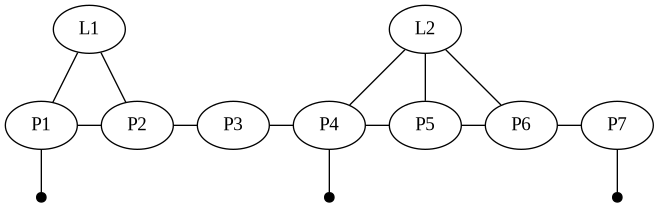
\includegraphics[width=\linewidth]{factor_graph.png}
  \caption{Example factor graph}
  \label{fig:factorgraph}
\end{figure}

In order to generate an initial trajectory estimate and local map of observed landmarks, we utilize a factor graph based SLAM method.
The variables in our factor graph consist of vehicle poses $X_t \in \mathrm{SE}(2)$ and landmark positions $L_n \in \mathbb{R}^2$.
Our vehicle data provides longitudinal velocity and yaw rate which can be combined into odometry factors $u_t \in \mathfrak{se}(2)$ between poses $X_t$ and $X_{t+1}$.
The GPS measurements $z_t \in \mathbb{R}^2$ are used as prior factors on the translational component of the current vehicle pose $X_t$ at the time that the measurement is obtained. Due to the difference in sampling rate of odometry and GPS data, not all poses will have an associated prior factor.
Each landmark observation consists of a landmark identifier $n$ and a distance to the landmark $v_i \in \mathbb{R}^2$ relative to the vehicle frame which is added as a factor between the pose $X_t$ at the time the measurement is obtained and the landmark location $L_n$.
An example simplified factor graph is shown in Figure \ref{fig:factorgraph}.

Variables and factors are added to the graph iteratively as new measurements become available.
To solve the factor graph we make use of the ISAM2 algorithm \cite{ref:isam} which internally converts the factor graph into a Bayes tree before optimizing. This approach allows for fast updates to variable estimates when adding new factors to the graph without the need for periodic batch relinearization or reordering.
Our final local map is the set of points of the best estimates of $L_n$ along with their semantic classes.

\subsection{Semantic Point Cloud Registration}
The odometry information used in the SLAM algorithm accumulates error over time. Without proper handling, this can cause the estimated trajectory to diverge from the true trajectory. The routine GPS signals received by the vehicle help to correct this (often they can give an acceptable level of localization by themselves), but these are also prone to error in certain circumstance, as discussed. This problem was alleviated by using a SICP algorithm to match the local map of landmarks, produced during the SLAM step, to a known global map of landmarks. Matching these landmarks produces a transformation from the estimated, locally observed landmark locations to the known, global locations. This transformation can then be applied to the estimated vehicle trajectory to improve the accuracy of the estimate. 

The matching of the local map to the global map uses a variation of the GICP algorithm presented by Parkison at al. \cite{cGICP}. This version has been modified to include the semantic labeling of the vehicle input sign data. The code itself is built upon the gicp\_SE3.m code written by Manni Ghaffari Jadidi \cite{cgicpse3}. This code was modified to include semantic labeling in the nearest neighbor search and sets the covariance normal to each point to the identity matrix to remove the functionality of looking at distributions around points near each other. Pseudo-code for the algorithm is shown below. One important note is that while the local and global maps are 2-dimensional (latitude and longitude) and the SLAM algorithm produces output in SE2, this function takes 3-dimensional data as an input, and produces a transformation in SE3. This was for the purpose of reusing the original code. Adding a zero vector as the third dimension, not calculating any translation along the z-axis, and only allowing rotations along the z-axis will have the same functionality.

\begin{algorithm}[ht]
\label{alg:sicpse3}
\begin{algorithmic}[1]
\Require  Initial Transformation T\textsuperscript{init}, target point cloud $\mathcal{X}_t$, source point cloud $\mathcal{X}_s$, semantic labels $\mathcal{S}$\\
T\textsuperscript{*} $\leftarrow$ T\textsuperscript{init}
	\While{not converged}
		\State T\textsuperscript{old} $\leftarrow$ T\textsuperscript{*} //set previous T to current T
		\State $\mathcal{I} = nnsearch{(\mathcal{X}_s, \mathcal{X}_t, \mathcal{S},  \mathrm{T\textsuperscript{old})}}$ // find nearest neighbor of same class in target for each source
		\State T\textsuperscript{*} $\leftarrow$ argmax\textsubscript{T $\in$ SE(3)} $f$\textsubscript{ICP}(T; $R|\mathcal{X}_t, \mathcal{X}_s, \mathcal{I})$ //optimize over SE(3) using ICP
		\If{d\textsubscript{SE(3)}(T\textsuperscript{old}, T\textsuperscript{*}) $ < \epsilon$}
			\State converged $\leftarrow$ true	
		\EndIf
	\EndWhile
	\State return T\textsuperscript{*}
\caption{Semantic ICP}
\end{algorithmic}
\end{algorithm}

The local and global landmark maps are used as the source and target point clouds, respectively. The initial transformation is estimated by using the previous GPS measurements. These most likely are not completely accurate but should be good enough for an initial estimate. For each landmark in the local map, we find the nearest neighbor \cite{cNN} of the same label in the global map. If a nearest neighbor of the same label cannot be found, or if it is further away than is allowable (tunable parameter), it is ignored for this iteration. Once a correlation between landmarks in the local map and target map have been found, a linear least squares problem is solved, which will produce a transformation. This transformation is then applied to the points in the local landmark map, and the process is repeated until convergence or the maximum number of iterations (tunable parameter) is reached. If the algorithm does not converge, or if it does converge, but the average distance between correlated landmarks in the transformed local map and the global map is too high (tunable paramater), then it will be ignored. Otherwise, the transformation is applied to the estimated trajectory to correct for the drift caused by noisy odometry and GPS data.

The SICP algorithm needs a relatively large number of observed landmarks in the local map in order to accurately perform the semantic map registration, or else there is a risk of the algorithm not converging or converging to the wrong transformation. Since the maps we are using include 3 dimensions, we will need at least six different landmarks, but it is preferable to have more than that. It takes time for the local landmark map to be created as the vehicle must drive around and discover new landmarks to be added to it. Additionally, for the SICP algorithm to be effective, those local landmarks must have corresponding landmarks of the same time in the local map. This necessitates that the SICP algorithm be run at a low frequency compared to the SLAM algorithm. This rate is heavily determined by the use case. A dense city, for example, will likely have more landmarks per area than a smaller city or rural area. In the case of this project, the SICP algorithm was run every 15 seconds of simulated time.


\section{RESULTS}

\begin{figure}[thpb]
  \centering
  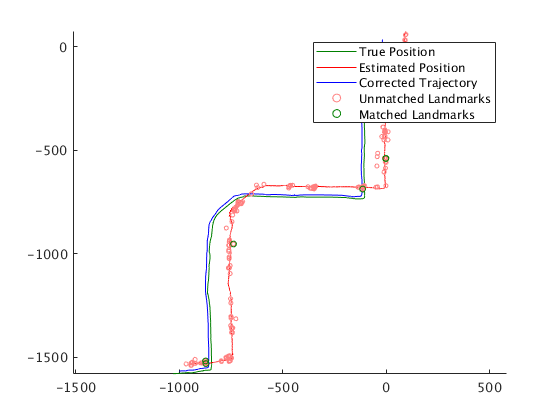
\includegraphics[width=\linewidth]{sim_results.png}
  \caption{Simulation results after observing 7 matched landmarks}
  \label{fig:simresults}
\end{figure}

\begin{figure}[thpb]
  \centering
  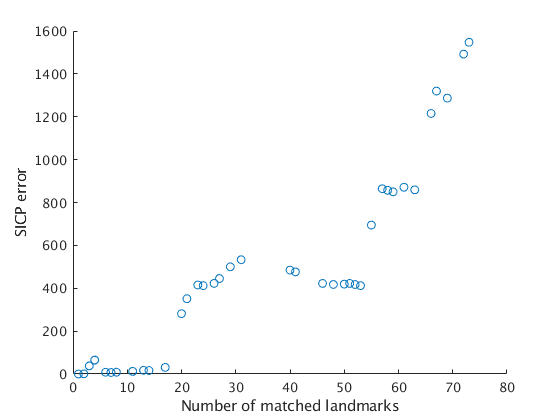
\includegraphics[width=\linewidth]{sicp_err.png}
  \caption{SICP error vs. Number of matched landmarks}
  \label{fig:sicperr}
\end{figure}

\begin{figure}[thpb]
  \centering
  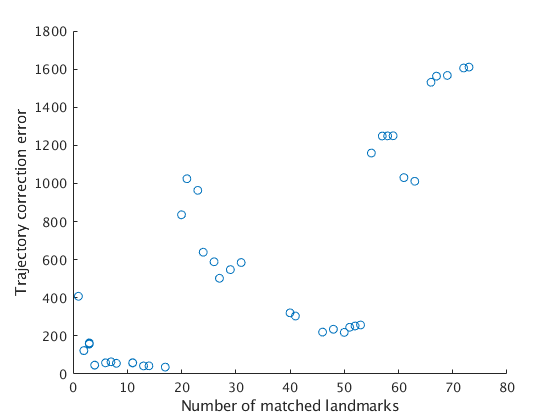
\includegraphics[width=\linewidth]{traj_err.png}
  \caption{Corrected trajectory error vs. Number of matched landmarks}
  \label{fig:trajerr}
\end{figure}

\begin{figure}[thpb]
  \centering
  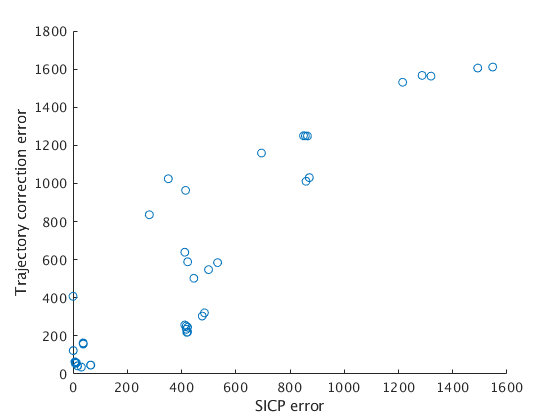
\includegraphics[width=\linewidth]{sicp_traj_err.png}
  \caption{Corrected trajectory error vs. SICP error}
  \label{fig:sicptrajerr}
\end{figure}

The data used to evaluate our method was taken from an hour long drive in downtown Chicago.
In order to test our methods ability to recover the true trajectory of the vehicle in the presence of bad GPS data, the collected GPS data was corrupted by adding an offset before passing it into the SLAM algorithm.
The GPS, odometry and landmark observation data was then replayed and passed into a MATLAB program implementing our algorithm.

In practice, many of the landmark types which were detected on the vehicle were not available in the map data. Although such landmarks can be useful in improving the trajectory estimate directly output from the SLAM algorithm, they are of no use when attempting to align the local and global maps.
As a result, a significant amount of driving time is required to obtain enough matching landmark observations in order to recover the true vehicle trajectory.

Figure \ref{fig:simresults} shows the results after finding 7 observed landmarks whose classes matched those found in the global map, which demonstrates that the true trajectory can be recovered with good accuracy.
Figure \ref{fig:sicperr} shows the error between the local map and global map after performing SICP alignment.
Figure \ref{fig:trajerr} shows the error between the corrected trajectory and the ground truth trajectory. This data shows that only a few points are necessary to recover the true trajectory. However, the dataset used had errors in some of the observed semantic classes which caused incorrect results from the SICP algorithm once those measurements were obtained.

Figure \ref{fig:sicptrajerr} shows the correlation between the SICP and corrected trajectory errors. There is a high correlation between the SICP error, which is observable without knowing the ground truth, and the error in the corrected trajectory. This indicates that the SICP error can be used as a good metric for determining whether or not the trajectory correction was successful.

\section{LIMITATIONS}


\subsection{Variability in Sign Data Between Data Sources}
The local and global road-sign data comes from different sources with different suppliers. These suppliers each have their own methods and specifications of detecting and representing road-sign data. The result of this is significant variability in the data between those sources.

The vehicle road-sign data consists of hundreds of different sign types while the global map data has a low density of sign data with much fewer sign types. The specification we had access to for the vehicle data road-sign types was not a complete list, as there were sign labels in the data that were not included in the documentation. In addition, sometimes, the vehicle road-sign data was incorrectly labeled, leading to incorrect correlation during the SICP algorithm. One particular sign that caused issues was the sign type 46, which is he label for a "No Turn on Red" sign. Many instances of these sign type had incorrect labels, which resulted in wrong correlation in the SICP algorithm and caused divergence from the correct solution. We fixed this by removing that sign type from our data. While this was an acceptable solution for the scope of this project, having correctly labeled signs is very important for future research.

Furthermore, there were only 15 matching road-sign labels from the vehicle data to the global map, even though the drive data has hundreds of different traffic sign types. The following are some of the traffic signs with matching correspondences between the vehicle data and global map: "Pedestrian Crossing", "STOP", "YIELD", "Road Narrows - Right", and "Slippery When Wet". Having access to more matching sign types would allow the SICP algorithm to better register the local landmark map to the global map.

\subsection{SICP Initial Guess}

A major limitation to the SICP algorithm is the algorithm's reliance on an accurate initial transform. If the GPS input data used for the initial transform is offset by too much, then the algorithm would find nearest neighbors in the wrong area, and converge to an incorrect transformation. This is especially true in a large city where the streets are likely to be arranged in a grid, with repeating patterns in the landmark map, such as stop signs at every intersection in an area. If the observed landmarks are arranged in a significantly similar pattern to the landmarks on adjacent streets, then even an offset of the size of one city block could cause a convergence to the wrong transformation. Additionally, minor changes in the angle of rotation between the local and global landmark maps can cause the algorithm to converge to the incorrect transform. This is also especially true when dealing with vehicle trajectories, as even a minor angle of rotation can cause drift that is hundreds or thousands of meters. The routine GPS input data helps to lessen the impact of this, as even noisy GPS data will give a good estimate of the direction traveled over the course of a drive through a city. 

\section{FUTURE WORK}

\subsection{Additional Landmark Information}
For this project, we only used road-signs as our landmarks for the SLAM and SICP algorithms. While this works well in some cases, it can also cause issues, as discussed. One major area of exploration is to expand the types of landmark information that is taken into account. This would hopefully further the ability of the SLAM algorithm to predict the correct trajectory and also give the SICP algorithm additional data points to use in the semantic registration. Below are some ideas of how this could be implemented:

\begin{itemize}
\item Expand the number of different sign types available in the global map to more closely match the number of sign types seen in the vehicle data. This could also include traffic lights.
\item Include sign types that are more unique, which would allow for better registration. These could include street signs that include the name of the street, storefront/business signs or signs that mark unique locations such as monuments or parks.
\item Add other road information that could help localize. This could include factors like the number of lanes on the road, road width, road curvature or road type.
\end{itemize}

\subsection{SICP}
The SICP algorithm used in this project was fairly simple, and could often converge to the incorrect location if the initial guess was off. While improving the available landmark information would lead to improvements in the SICP algorithm, improving the SICP algorithm could be a potential major increase the performance of this function. Below are some ideas of how this could be implemented:

\begin{itemize}
\item Perform semantic GICP instead of ICP to consider the covariance of normal vectors to distributions of landmarks that are near each other. Road-signs will generally follow a specific distribution, with signs near or on the road, and facing the direction of travel on that road. This fact could be used when registering the local landmark map to the global landmark map to allow better correlation between landmarks. This idea of semantic GICP is discussed in Parison et al. \cite{cGICP}
\item Instead of running the SICP algorithm once every iteration, it could be run multiple times with different initial guesses. For each resulting transformation, the average distance between the transformed local landmarks and the global landmarks could be computed, and the transformation with the lowest average distance away could be taken.
\item Research other ICP algorithms that have been developed by researchers that already improve upon the ICP algorithm used here. For example, Szymon Rusinkiewicz and Marc Levoy of Stanford University \cite{ref:futurework} have developed an ICP algorithm that uses a random, weighted, sampling of the point clouds and a different method for determining correlation instead of closes point as we used in this project.
\item Use known geographical information to infer potential paths the vehicle could take. For example, if we know that the downtown of a city has only roads in a grid going north-south and east-west, then we know that the trajectory must be one of those directions. A probabilistic method of determining which path the vehicle could turn could be used to register points more accurately.
\end{itemize}



\addtolength{\textheight}{-12cm}   % This command serves to balance the column lengths
                                  % on the last page of the document manually. It shortens
                                  % the textheight of the last page by a suitable amount.
                                  % This command does not take effect until the next page
                                  % so it should come on the page before the last. Make
                                  % sure that you do not shorten the textheight too much.

%%%%%%%%%%%%%%%%%%%%%%%%%%%%%%%%%%%%%%%%%%%%%%%%%%%%%%%%%%%%%%%%%%%%%%%%%%%%%%%%




\begin{thebibliography}{99}

\bibitem{cHERE} “Automotive Technologies.” HERE. Accessed May 1, 2020. https://www.here.com/products/automotive.
\bibitem{cGICP} Parkison et al. Semantic Iterative Closest Point through Expectation-Maximization. http://robots.engin.umich.edu/publications/sparkison-2018a.pdf
\bibitem{cgicpse3} Maani Ghaffari Jadidi (2020) sicp\_se3.m [algorithm] https://umich.instructure.com/courses/344063/files/folder/code/gicp
\bibitem{cNN} “K-Nearest Neighbors Algorithm.” Wikipedia. Wikimedia Foundation, April 14, 2020. https://en.wikipedia.org/wiki/K-nearest\_neighbors\_algorithm.
\bibitem{ref:isam} M. Kaess, 'iSAM2: Incremental Smoothing and Mapping Using the Bayes Tree,' Intl. J. of Robotics Research, 31(2), 216-235.
\bibitem{ref:futurework}'Efficient Variants of the ICP Algorithm', by Szymon Rusinkiewicz and Marc Levoy, Stanford University.


\end{thebibliography}

\end{document}
